

\chapter{Classes and functions}
\label{time}

Now that we know how to create new types, the next
step is to write functions that take programmer-defined objects
as parameters and return them as results.  In this chapter I
also present ``functional programming style'' and two new
program development plans.

Code examples from this chapter are available from
\url{http://thinkpython2.com/code/Time1.py}.
Solutions to the exercises are at
\url{http://thinkpython2.com/code/Time1_soln.py}.


\section{Time}
\label{isafter}

As another example of a programmer-defined type, we'll define a class
called {\tt Time} that records the time of day.  The class definition
looks like this: \index{programmer-defined type}
\index{type!programmer-defined} \index{Time class} \index{class!Time}

\begin{verbatim}
class Time:
    """Represents the time of day.

    attributes: hour, minute, second
    """
\end{verbatim}
%
We can create a new {\tt Time} object and assign
attributes for hours, minutes, and seconds:

\begin{verbatim}
time = Time()
time.hour = 11
time.minute = 59
time.second = 30
\end{verbatim}
%
The state diagram for the {\tt Time} object looks like Figure~\ref{fig.time}.
\index{state diagram}
\index{diagram!state}
\index{object diagram}
\index{diagram!object}

As an exercise, write a function called \verb"print_time" that takes a
Time object and prints it in the form {\tt hour:minute:second}.
Hint: the format sequence \verb"'%.2d'" prints an integer using
at least two digits, including a leading zero if necessary.

Write a boolean function called \verb"is_after" that
takes two Time objects, {\tt t1} and {\tt t2}, and
returns {\tt True} if {\tt t1} follows {\tt t2} chronologically and
{\tt False} otherwise.  Challenge: don't use an {\tt if} statement.

\begin{figure}
\centerline
{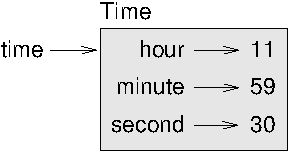
\includegraphics[scale=0.8]{../source/figs/time.pdf}}
\caption{Object diagram.}
\label{fig.time}
\end{figure}


\section{Pure functions}
\index{prototype and patch}
\index{development plan!prototype and patch}

In the next few sections, we'll write two functions that add time
values.  They demonstrate two kinds of functions: pure functions and
modifiers.  They also demonstrate a development plan I'll call {\bf
  prototype and patch}, which is a way of tackling a complex problem
by starting with a simple prototype and incrementally dealing with the
complications.

Here is a simple prototype of \verb"add_time":

\begin{verbatim}
def add_time(t1, t2):
    sum = Time()
    sum.hour = t1.hour + t2.hour
    sum.minute = t1.minute + t2.minute
    sum.second = t1.second + t2.second
    return sum
\end{verbatim}
%
The function creates a new {\tt Time} object, initializes its
attributes, and returns a reference to the new object.  This is called
a {\bf pure function} because it does not modify any of the objects
passed to it as arguments and it has no effect,
like displaying a value or getting user input,
other than returning a value.
\index{pure function}
\index{function type!pure}

To test this function, I'll create two Time objects: {\tt start}
contains the start time of a movie, like {\em Monty Python and the
Holy Grail}, and {\tt duration} contains the run time of the movie,
which is one hour 35 minutes.
\index{Monty Python and the Holy Grail}

\verb"add_time" figures out when the movie will be done.

\begin{verbatim}
>>> start = Time()
>>> start.hour = 9
>>> start.minute = 45
>>> start.second =  0

>>> duration = Time()
>>> duration.hour = 1
>>> duration.minute = 35
>>> duration.second = 0

>>> done = add_time(start, duration)
>>> print_time(done)
10:80:00
\end{verbatim}
%
The result, {\tt 10:80:00} might not be what you were hoping
for.  The problem is that this function does not deal with cases where the
number of seconds or minutes adds up to more than sixty.  When that
happens, we have to ``carry'' the extra seconds into the minute column
or the extra minutes into the hour column.
\index{carrying, addition with}

Here's an improved version:

\begin{verbatim}
def add_time(t1, t2):
    sum = Time()
    sum.hour = t1.hour + t2.hour
    sum.minute = t1.minute + t2.minute
    sum.second = t1.second + t2.second

    if sum.second >= 60:
        sum.second -= 60
        sum.minute += 1

    if sum.minute >= 60:
        sum.minute -= 60
        sum.hour += 1

    return sum
\end{verbatim}
%
Although this function is correct, it is starting to get big.
We will see a shorter alternative later.


\section{Modifiers}
\label{increment}
\index{modifier}
\index{function type!modifier}

Sometimes it is useful for a function to modify the objects it gets as
parameters.  In that case, the changes are visible to the caller.
Functions that work this way are called {\bf modifiers}.
\index{increment}

{\tt increment}, which adds a given number of seconds to a {\tt Time}
object, can be written naturally as a
modifier.  Here is a rough draft:

\begin{verbatim}
def increment(time, seconds):
    time.second += seconds

    if time.second >= 60:
        time.second -= 60
        time.minute += 1

    if time.minute >= 60:
        time.minute -= 60
        time.hour += 1
\end{verbatim}
%
The first line performs the basic operation; the remainder deals
with the special cases we saw before.
\index{special case}

Is this function correct?  What happens if {\tt seconds}
is much greater than sixty?

In that case, it is not enough to carry once; we have to keep doing it
until {\tt time.second} is less than sixty.  One solution is to
replace the {\tt if} statements with {\tt while} statements.  That
would make the function correct, but not very efficient.  As an
exercise, write a correct version of {\tt increment} that doesn't
contain any loops.

Anything that can be done with modifiers can also be done with pure
functions.  In fact, some programming languages only allow pure
functions.  There is some evidence that programs that use pure
functions are faster to develop and less error-prone than programs
that use modifiers.  But modifiers are convenient at times,
and functional programs tend to be less efficient.

In general, I recommend that you write pure functions whenever it is
reasonable and resort to modifiers only if there is a compelling
advantage.  This approach might be called a {\bf functional
programming style}.
\index{functional programming style}

As an exercise, write a ``pure'' version of {\tt increment} that
creates and returns a new Time object rather than modifying the
parameter.


\section{Prototyping versus planning}
\label{prototype}
\index{prototype and patch}
\index{development plan!prototype and patch}
\index{planned development}
\index{development plan!designed}

The development plan I am demonstrating is called ``prototype and
patch''.  For each function, I wrote a prototype that performed the
basic calculation and then tested it, patching errors along the
way.

This approach can be effective, especially if you don't yet have a
deep understanding of the problem.  But incremental corrections can
generate code that is unnecessarily complicated---since it deals with
many special cases---and unreliable---since it is hard to know if you
have found all the errors.

An alternative is {\bf designed development}, in which high-level
insight into the problem can make the programming much easier.  In
this case, the insight is that a Time object is really a three-digit
number in base 60 (see \url{http://en.wikipedia.org/wiki/Sexagesimal}.)!  The
{\tt second} attribute is the ``ones column'', the {\tt minute}
attribute is the ``sixties column'', and the {\tt hour} attribute is
the ``thirty-six hundreds column''.
\index{sexagesimal}

When we wrote \verb"add_time" and {\tt increment}, we were effectively
doing addition in base 60, which is why we had to carry from one
column to the next.
\index{carrying, addition with}

This observation suggests another approach to the whole problem---we
can convert Time objects to integers and take advantage of the fact
that the computer knows how to do integer arithmetic.

Here is a function that converts Times to integers:

\begin{verbatim}
def time_to_int(time):
    minutes = time.hour * 60 + time.minute
    seconds = minutes * 60 + time.second
    return seconds
\end{verbatim}
%
And here is a function that converts an integer to a Time
(recall that {\tt divmod} divides the first argument by the second
and returns the quotient and remainder as a tuple).
\index{divmod}

\begin{verbatim}
def int_to_time(seconds):
    time = Time()
    minutes, time.second = divmod(seconds, 60)
    time.hour, time.minute = divmod(minutes, 60)
    return time
\end{verbatim}
%
You might have to think a bit, and run some tests, to convince
yourself that these functions are correct.  One way to test them is to
check that \verb"time_to_int(int_to_time(x)) == x" for many values of
{\tt x}.  This is an example of a consistency check.
\index{consistency check}

Once you are convinced they are correct, you can use them to
rewrite \verb"add_time":

\begin{verbatim}
def add_time(t1, t2):
    seconds = time_to_int(t1) + time_to_int(t2)
    return int_to_time(seconds)
\end{verbatim}
%
This version is shorter than the original, and easier to verify.  As
an exercise, rewrite {\tt increment} using \verb"time_to_int" and
\verb"int_to_time".

In some ways, converting from base 60 to base 10 and back is harder
than just dealing with times.  Base conversion is more abstract; our
intuition for dealing with time values is better.

But if we have the insight to treat times as base 60 numbers and make
the investment of writing the conversion functions (\verb"time_to_int"
and \verb"int_to_time"), we get a program that is shorter, easier to
read and debug, and more reliable.

It is also easier to add features later.  For example, imagine
subtracting two Times to find the duration between them.  The
naive approach would be to implement subtraction with borrowing.
Using the conversion functions would be easier and more likely to be
correct.
\index{subtraction with borrowing}
\index{borrowing, subtraction with}
\index{generalization}

Ironically, sometimes making a problem harder (or more general) makes it
easier (because there are fewer special cases and fewer opportunities
for error).


\section{Debugging}
\index{debugging}

A Time object is well-formed if the values of {\tt minute} and {\tt
second} are between 0 and 60 (including 0 but not 60) and if
{\tt hour} is positive.  {\tt hour} and {\tt minute} should be
integral values, but we might allow {\tt second} to have a
fraction part.
\index{invariant}

Requirements like these are called {\bf invariants} because
they should always be true.  To put it a different way, if they
are not true, something has gone wrong.

Writing code to check invariants can help detect errors
and find their causes.  For example, you might have a function
like \verb"valid_time" that takes a Time object and returns
{\tt False} if it violates an invariant:

\begin{verbatim}
def valid_time(time):
    if time.hour < 0 or time.minute < 0 or time.second < 0:
        return False
    if time.minute >= 60 or time.second >= 60:
        return False
    return True
\end{verbatim}
%
At the beginning of each function you could check the
arguments to make sure they are valid:
\index{raise statement}
\index{statement!raise}

\begin{verbatim}
def add_time(t1, t2):
    if not valid_time(t1) or not valid_time(t2):
        raise ValueError('invalid Time object in add_time')
    seconds = time_to_int(t1) + time_to_int(t2)
    return int_to_time(seconds)
\end{verbatim}
%
Or you could use an {\bf assert statement}, which checks a given invariant
and raises an exception if it fails:
\index{assert statement}
\index{statement!assert}

\begin{verbatim}
def add_time(t1, t2):
    assert valid_time(t1) and valid_time(t2)
    seconds = time_to_int(t1) + time_to_int(t2)
    return int_to_time(seconds)
\end{verbatim}
%
{\tt assert} statements are useful because they distinguish
code that deals with normal conditions from code
that checks for errors.


\section{Glossary}

\begin{description}

\item[prototype and patch:] A development plan that involves
writing a rough draft of a program, testing, and correcting errors as
they are found.
\index{prototype and patch}

\item[designed development:] A development plan that involves
high-level insight into the problem and more planning than incremental
development or prototype development.
\index{designed development}

\item[pure function:] A function that does not modify any of the objects it
receives as arguments.  Most pure functions are fruitful.
\index{pure function}

\item[modifier:] A function that changes one or more of the objects it
  receives as arguments.  Most modifiers are void; that is, they
  return {\tt None}.  \index{modifier}

\item[functional programming style:] A style of program design in which the
majority of functions are pure.
\index{functional programming style}

\item[invariant:] A condition that should always be true during the
execution of a program.
\index{invariant}

\item[assert statement:] A statement that check a condition and raises
an exception if it fails.
\index{assert statement}
\index{statement!assert}

\end{description}


\section{Exercises}

Code examples from this chapter are available from
\url{http://thinkpython2.com/code/Time1.py}; solutions to the
exercises are available from \url{http://thinkpython2.com/code/Time1_soln.py}.

\begin{exercise}

Write a function called \verb"mul_time" that takes a Time object
and a number and returns a new Time object that contains
the product of the original Time and the number.

Then use \verb"mul_time" to write a function that takes a Time
object that represents the finishing time in a race, and a number
that represents the distance, and returns a Time object that represents
the average pace (time per mile).
\index{running pace}

\end{exercise}


\begin{exercise}
\index{datetime module}
\index{module!datetime}

The {\tt datetime} module provides {\tt time} objects
that are similar to the Time objects in this chapter, but
they provide a rich set of methods and operators.  Read the
documentation at \url{http://docs.python.org/3/library/datetime.html}.

\begin{enumerate}

\item Use the {\tt datetime} module to write a program that gets the
  current date and prints the day of the week.

\item Write a program that takes a birthday as input and prints the
  user's age and the number of days, hours, minutes and seconds until
  their next birthday.
\index{birthday}

\item For two people born on different days, there is a day when one
  is twice as old as the other.  That's their Double Day.  Write a
  program that takes two birthdays and computes their Double Day.

\item For a little more challenge, write the more general version that
  computes the day when one person is $n$ times older than the other.
\index{Double Day}

\end{enumerate}

Solution: \url{http://thinkpython2.com/code/double.py}

\end{exercise}